\documentclass[../main.tex]{subfiles}

\usepackage{listings}
\usepackage{setspace}

\begin{document}

\chapter*{Chapter 12: Hyperbolic and Parabolic Partial
Differential Equations}

\section*{12.1: EXAMPLES AND CONCEPTS OF HYPERBOLIC PDE'S}

In the last chapter, we discussed in some detail the heat and Laplace's equations,
which are prototypes for parabolic and elliptic PDEs, respectively. We would like
now to introduce some concepts and theory for the wave equation, which is the
prototype for hyperbolic equations. The wave equation models many natural
phenomena, including gas dynamics (in particular, acoustics), vibrating solids and
electromagnetism. It was first studied in the eighteenth century to model vibrations
of strings and columns of air in organ pipes. Several mathematicians contributed
to these initial studies, including Taylor, Euler, and Jean D'Alembert, about whom
we will say more shortly. Subsequently in the nineteenth century, the wave
equation was used to model elasticity as well as sound and light waves, and in the
twentieth century, it has been used in quantum mechanics and relativity and most
recently in such fields as superconductivity and string theory. In general, the
wave equation has a time variable t and any number of space variables JC, y, z,...
and takes the form

\begin{equation}
u_u=c^2 \vartriangle u=c^2(u_{xx}+u_{yy}+...) 
\end{equation}

where c is a positive constant and the Laplace operator on the right is with respect
to all of the space variables. Modifications of this equation have been successfully
used to model numerous physical waves and wavelike phenomena. In two space
variables, for example, allowing for a variable wave speed due to depth
differences in an ocean, the PDE:
$u_u=\nabla \cdot[H(x,y,t) \nabla u] + H_u$
has been used to
model large destructive ocean waves. 
\footnote 
{ The symbol $\nabla$, read as "nabla" or "del," is used to represent the gradient operator, which is the
vector of all partial derivatives of a function. Thus for a function of two variables 
$f(x,y)$ , $\nabla f=\nabla  f(x,y)=(f_x(x,y), f_y(x,y))$
. The large dot represents the vector dot product, so in long form: 
$\nabla \cdot [H(x,y,t)\nabla u]= (\partial_x, \partial_y)\cdot (Hu_x, Hu_y)=\partial_x (Hu_x)+\partial(Hu_y)$. In particular, when  $H\equiv 1$ we have $\nabla \cdot [\nabla u]=\partial_x (u_x)+ \partial_y(u_y)=u_{xx}+u_{yy}=\triangle u $, another way to write the Laplacian of u. Such notations
are very common in the literature for partial differential equations involving several space variables.}
In such an application, the function H is the
depth of the ocean at space coordinates (longitude and latitude) (JC, y) and at time /.
The latter term corresponds to the changes in depth due to underwater landslides.
For more on this and other applications of this variable media wave equation, we
mention the text [Lan-99].

Much of the general theory of hyperbolic PDEs is well represented by that for the \textbf{one-dimensional wave equation} $(u = u(x,t)$ depends on time / and one space
variable x\ so we proceed now to introduce it through its historical model of a
vibrating string and present some of the theory. At the end of the section we
indicate some differences and similarities of higher-dimensional waves to onedimensional waves. 
\\

We consider a small segment of taut string having length As and uniform tension
T that is acted on by a vertical force q, as shown in Figure 12.1. 
\\

We assume that the string is displaced only in the vertical (transverse) direction,
and let $u(x,t)$ denote the y-coordinate of the string at horizontal coordinate x at the
time t. If we let $\rho$ denote the mass density (mass per unit length) of the string
(assumed constant), then Newton's second law (F = ma) gives us that 
$$-T sin \Theta +T sin (\Theta +\vartriangle \Theta )+q\vartriangle s \rho \triangle su_u (x,t) $$,  
where the first two terms represent the vertical component of the internal elastic
forces acting on the segment of string.

\begin{figure}[H]
	\centering
	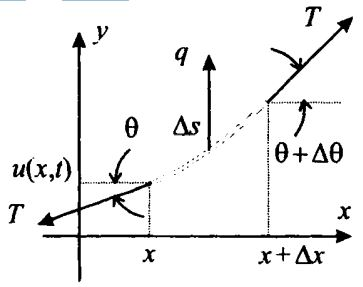
\includegraphics[width=0.4\linewidth]{ch12_1}
	\caption{\textsf{: A segment of a uniformly taut string having tension Tand external load g.
The string is displaced vertically only, and u(x,t) is the vertical level of the string at time /
and horizontal position x .}}
	\label{pfig:ch12_1}
\end{figure}

For small deflections in the string, we have 
$\triangle s\thickapprox \triangle x$
 and also  
 $sin(\theta) \thickapprox \theta \thickapprox u_x (x,t)$
  In the limit as As -» 0, this brings us to

\begin{equation}
Tu_{xx}+q =\rho u_u ,u=u()x,t 
\end{equation}


which is the \textbf{one-dimensional wave equation with external load term} q. In case
q = 0, this reduces to the one-dimensional wave equation (1) with 
$c=(T/\rho)^{1/2}$
. It turns out that this parameter c is the speed at which the wave (i.e., any solution
of the equation) propagates. This will be made clear shortly. Intuitively, it makes
sense that the speed of any disturbance on a string should increase along with the
tension and decrease for heavier strings. For a derivation of wave equations for
strings under more general hypotheses we refer to the article by S. Antman [Ant80] or Chapter 3 of the textbook by Kevorkian [Kev-00].


\begin{wrapfigure}{l}{0.25\textwidth}
    \centering
    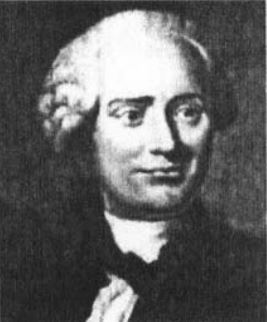
\includegraphics[width=0.25\textwidth]{ch12_2}
   \caption{\textsf{Jean Le Rond
D'Alembert (1717-1783),
French mathematician.}}
   \label{fig:ch12_2}
\end{wrapfigure}


The general solution of the one-dimensional wave
equation was first derived by the French
mathematician Jean D'Alembert. 
\footnote 
{Jean D'Alembert was born in Paris as an illegitimate child of a former nun while the father was out of
the country. Unable to support her son, his mother left him on the steps of a church. The infant was
quickly found and taken to an orphanage. He was baptized as Jean Le Rond, after the name of the
church where he was found. When the infant's father returned to Paris, he arranged for Jean to be
adopted by a married couple, who were friends of his. His adoptive parents brought him up well. He
studied law and earned a law degree. He soon decided that mathematics was his true passion and
studied it on his own. Although mostly self-taught, D'Alembert became an eminent mathematician and
scholar in the same league with the likes of Euler, Laplace, and Lagrange. He made significant
contributions to partial differential equations and his elegant methods, including his solution to the
wave equation, very much impressed Euler. Frederick II (King of Prussia) offered D'Alembert the
presidency of the prestigious Berlin Academy, a position which he declined. He was quite an eloquent
and well-rounded scholar and he made significant contributions to Diderot's famous encyclopedia.
Apparently, D'Alembert was prone to argumentation and his disputes with other contemporary
mathematicians caused him some professional difficulties on several occasions.}
 D'Alemberfs
derivation is simple and elegant and the form of
the solution will give many insights into qualitative
aspects of wave equations. It begins by
introducing the new variables: 

\begin{equation}
\xi=x-ct, \eta=x+ct 
\label{eq:eps}
\end{equation}

We may now think of u as either a function of (x,t)
or of $(\xi,\eta )$. When we use the chain rule to
translate the wave equation (1) into a PDE with
respect to the new variables $(\xi,\eta )$ something
very nice will happen. The resulting PDE will be
extremely easy to solve for the general solution. Applied using (3), the chain rule
gives the following: 

$$u_x = u_\xi \xi_x + u_\eta \eta_x = u_\xi u_\eta$$
\begin{equation}
u_t =u_\xi \xi_t +u_\eta \eta_t =-cu_\xi+cu_\eta
\label{eq:eps}
\end{equation}
\\
\\
\\
\\
In the same fashion, if we differentiate once again, we arrive at
\begin{equation}
u_{xx} =u_{\xi \xi}+2u_{\xi \eta}+u_{\eta \eta} , u_u = c^2(u{\xi \xi}-2u_{\xi \eta}+ u_{\eta \eta})  
\label{eq:eps}
\end{equation}
When we substitute equations (5) into the one-dimensional wave equation (1), we
obtain the following version of the wave equation in the new variables $(\xi ,\eta)$ : 

\begin{equation}
u_{\xi \eta}=0.
\label{eq:eps}
\end{equation}
This PDE is very easy to solve, by "integrating" twice. Since it says that $\partial /\partial \eta(u_\xi)=0,$ we can integrate with respect to $\eta$ to get $u_\xi=(F\xi)$,where


$F(\xi)$  is an arbitrary function of $\xi$ Next we integrate again, this time with respect
to $\xi$ , to conclude that

\begin{equation}
u(\xi,\eta)=f(\xi)+g(\eta),
\label{eq:eps}
\end{equation}
where $f(\xi)$ and $g(\eta)$ are arbitrary functions of the indicated variables. (Note  $f(\xi)$ is an antiderivative of $F(\xi)$) Translating back to the original variables
using (3) gives us the following general solution of the wave equation:

\begin{equation}
u(x,t)=f(x-ct)+g(x + ct),
\label{eq:eps}
\end{equation}
where $f$ and $g$ are arbitrary functions (with continuous second derivatives). We
point out that each term in (8) represents a wave propagating along the x-axis with
speed c. For example,  $f(x-ct)$  is constant on lines of the form $x = ct$. As time $t$
advances, values of x must also increase to maintain the same value of $f$ (disturbance). Thus the first term represents a wave that propagates in the positive
jc-direction with speed c (right traveling wave). Similarly, the term
$g(x + ct)$ represents a left-traveling wave Both waves travel without distortion
(i.e., the profile of either one of them / units of time later will be the exact same
profile, but shifted to the left or right ct units along the x-axis.)

\begin{figure}[H]
	\centering
	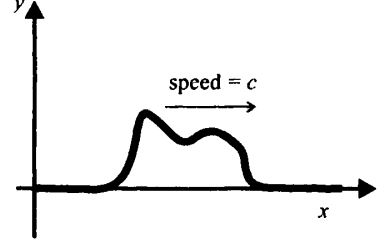
\includegraphics[width=0.4\linewidth]{ch12_3}
	\caption{\textsf{: A right-propagating pulse $f(x - ct$). The general solution (8) of the onedimensional wave equation $u_\eta = c^2 u_{xx}$
also includes a left-propagating pulse. Both
wavefronts propagate without distortion.}}
	\label{pfig:ch12_3}
\end{figure}

D'Alembert went on further with his general solution (8), formulating and
solving a well-posed problem for the one-dimensional wave equation. We
consider a very long string and so consider the one-dimensional wave equation on
the space range $ -\infty <x< \infty$ o, and the time range $ 0 \leqslant t < \infty $ 
Unlike with the heat
equation, it is quite clear from (8) that merely specifying the wave profile W(JC,0) at
time / = 0 is not sufficient to determine a unique solution. Indeed, the initial wave
could come from a single left-moving wave, a single right-moving wave, or more
generally could be made up as a superposition of two waves each moving in
different directions.If we specify both the initial wave profile $u(x,0)$ and its
initial velocity $u_t(x,0)$ ) , then this together with the wave equation will give a well-


posed problem. These initial boundary conditions are often referred to as \textbf{Cauchy
boundary conditions}  (or \textbf{Cauchy boundary data}) Thus the \textbf{Cauchy problem
for the wave equation} is summarized as follows: 

\begin{equation}
\left\{\begin{array}{ll}
(PDE) u_\eta=c^2u_{xx}, -\infty<x<\infty, 0<t<\infty, u=u(x,t)\\
(BC's) u(x,0)=\phi(x), u_t(x,0)=v(x)-\infty<x<\infty ,=\leqslant \infty
\end{array} \right.
\label{eq:eps}
\end{equation}
This highlights an important general difference between elliptic PDEs versus
hyperbolic PDEs. Recall from the last chapter that for elliptic PDEs, simply
specifying the value of the solution on the boundary of the domain (Dirichlet
boundary conditions) resulted in a well-posed problem. For hyperbolic PDEs,
more information is needed for the problem to be well posed. We now state
d'Alembert's solution of this Cauchy problem: 
\\
\\
\textbf{THEOREM 12.1:}
(\emph{D 'Alembert 's Solution of the Cauchy Problem?}\footnote
{ In applications, it is convenient to allow functions $\phi(x)$ and $v(x)$ for initial data which may violate
the technical assumptions of having the required derivatives at all values of x. Often there are a finite
set of values (singularities) of x at which either $\phi(x)$ or $v(x)$ may not even be defined or their
derivatives may not exist. Such singularities do not pose any serious problems for d'Alembert's
solution, but they will give rise to corresponding singularities in the solution at all future time values.
See, for example, the initial profile of Figure 12.4 $(\phi(x))$ for a wave problem.  This function has
singularities at the three points where there are sharp corners in the graph $x = -1 , 0, 1$. Future profiles
in the solution shown in Figure 12.5 show also the presence of such singularities. Recall that for
solutions of heat equations that were seen in the last chapter, singularities arising from discontinuities
in an initial temperature distribution or its derivative immediately got smoothed out as time advanced.
This is one of the major distinguishing features between hyperbolic versus parabolic PDE's. In the
former, singularities are preserved and propagate, while in parabolic PDE's, initial singularities
disappear as soon as time becomes positive.} 
Suppose that
the function $\phi(x)$ has a continuous second derivative and $v(x)$ has a continuous
first derivative on the whole real line. Then the Cauchy problem (9) for the onedimensional wave equation has the unique solution given by 

\begin{equation}
u(x,t)=\dfrac{1}{2} \phi(x+ct)+\phi(x-ct)+\dfrac{1}{2c} \int_{x-ct}^{x+ct} v(s)ds
\end{equation}
Proof: Substitution of the general solution (8) into the BCs of (9) produces (put /
= 0): 
$$\phi(x)=f(x)+g(x), and v(x)=-cf'(x)+cg'(x)$$
Integrating the second equation and dividing by c gives:$(1/c) \int_{0}^{x} V(s)ds=g(x)-f(x)$
(Since $f(x)$ and $g(x)$ are arbitrary functions we can assume that the
constant of integration is zero.) This last equation together with the first of the
original pair are easily solved to give:

$$f(x)=\dfrac{1}{2}[\phi(x)-\dfrac{1}{c}] \int_{0}^{x} V(s)ds] , g(x)=\dfrac{1}{2}[\phi(x)+\dfrac{1}{c}] \int_{0}^{x} V(s)ds]$$

Substituting these formulas into (8) now lets us write the solution as: 
$$f(x-ct) + g(x + ct)=\dfrac{1}{2} [\phi(x+ct)+\phi(x-ct)]+\dfrac{1}{2c} [-\int_{0}^{x-ct} v(s)ds+\int_{0}^{x+ct} v(s)ds]'$$
which equals the expression in (10). 
\\

We emphasize that the foregoing analysis was only for one-dimensional waves
on an infinite string. Of course, infinite strings do not exist, but for long strings, or
for modeling disturbances on finite strings for limited time intervals, the above
analysis can lead to useful insights. It is rare to have such an explicit analytical
general solution. Soon we will consider boundary conditions that will require
nonanalytical numerical methods, and finite-difference methods will be employed
as in the last chapter. For now, let us get some hands-on experience with
traveling waves. In the following example, we will get MATLAB to create a
series of snapshots of a solution of a natural wave problem.
\\
\\ 
\textbf{EXAMPLE 12.1:} (A Plucked Infinite String) Consider what happens to a long
string that is plucked with three fingers as shown in Figure 12.4 and then released
(at time $t = 0$). Assume that the units are chosen so that wave speed $c=(T/ \phi)^1/2$ equals 1. Using d'Alembert's solution, get MATLAB to create a series of
snapshots of the wave profiles for each of the seven times starting with time $t = 0$
and advancing to $t = 3$ in increments of 0.5. 
\begin{figure}[H]
	\centering
	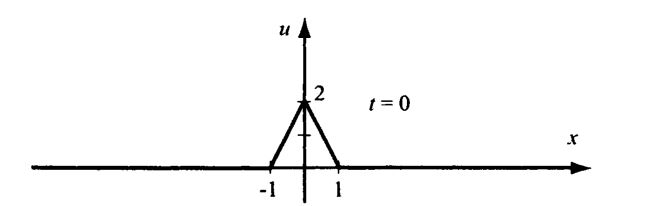
\includegraphics[width=0.6\linewidth]{ch12_4}
	\caption{\textsf{ Initial profile for the plucked string of Example 12.1.}}
	\label{pfig:ch12_4}
\end{figure}

SOLUTION: In the Cauchy problem (9), we put $c = 1$, and $v(x) = 0$ (since at
time $t = 0$, the three-finger plucked string is released with no initial velocity).
From Figure 12.4, we can write the initial profile of the string as

$\phi(x)=
\begin{cases} 2-2\vert x\vert,  ~~~~for~ \vert x\vert \leqslant 1\\
0, for  ~~~~~~~~~~~~~~~\vert x\vert\geqslant 1
\end{cases}$
It is not too difficult to analyze the resulting wave
[0, for |JC| > 1
propagation analytically using Theorem 12.1, but a MATLAB code can be easily
written to produce snapshots and/or movies of this and more complicated waves.
Since an inline function construction is not appropriate for functions whose
formulas change, we first construct an M-file for the function $\phi(x):$

\begin{verbatim}
function y = EX121(x)
if abs(x)<l, y=2-2*abs(x);
else y=0;
end
\end{verbatim}
Using this M-file in the following code, we create relevant vectors to produce the
snapshots, and we use the \textit{subplot} command to conveniently collect all of the
profiles in a single figure. The resulting MATLAB plot window is reproduced in
Figure 12.5. 

\begin{lstlisting}
>> x=-5:.01:5;
>> counter =1;
>> for t=0:.5:3;
		xl=x+t; x2=x-t;
		for i=l:1001
			u(i)=.5*(EX12_l(xl(i))+EX12_l(x2(i)));
		end
		subplot(7,1,counter)
		plot(x,u)
		hold on
		axis ([-5 5 -1 3]) rsWo fix a good axis range.
		counter=counter+l;
	end 
\end{lstlisting}

EXERCISE FOR THE READER 12.1: Following the procedure for making a
movie in Section 7.2, get MATLAB to create a movie of the solution of the wave
problem of Example 12.1 for the time range $0</<4$ . Play it back at varying
speeds (and perhaps with varying repetitions).\\
\\
EXERCISE FOR THE READER : (a) Write a function M-file:

\begin{verbatim}
function [] = dalembert(c,step, finaltime, phi, nu, range),  
\end{verbatim}
for creating a series of snapshots for the solution of the one-dimensional wave
problem (9). The inputs should be: a positive number c for the wave speed, a
positive number \texttt{step}  for the time steps of the snapshots, and another positive
number \texttt{ finaltime } for the time limit of the snapshots. Also, the initial data of
the problem will be inputted as two inline or M-file functions \textbf{phi} and \texttt{nu} The
last input variable is a 4x1 vector \texttt{range} for the xy-axis range to use in the
snapshots. There will be no output variables, but the program will produce a
graphic of snapshots of the Cauchy problem (9) starting at time t = 0 and
continuing in increments of \texttt{step} until \texttt{ finaltime } e is exceeded.\\
(b) Run your program using the data of Example 12.1.\\
(c) Run your program on the "hammer blow" problem that consists of the Cauchy
problem (9) (for the wave equation) with c = 1, <p(x) = 0, and
$V(x)
\begin{cases} 
1, for \vert x \vert \leqslant 1\\
0, for  \vert x\vert\geqslant 1
\end{cases}$
Create a series of snapshots of the solution from / = 0 to t = 5 in increments of / = 0.5.\\
(d) Use your program to help you estimate the length of time it takes for the
disturbances of the waves of both parts (b) and (c) above to reach an observer at

position JC = 10. How do your answers fit in with the previously mentioned fact
that the waves in making up d'Alembert's general solution of the wave equation
travel at speed c (here c = 1)? 
\begin{figure}[H]
	\centering
	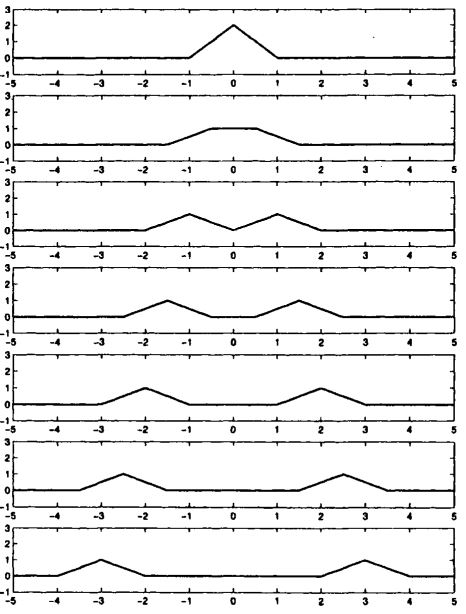
\includegraphics[width=0.6\linewidth]{ch12_5}
	\caption{\textsf{ Progressive snapshots of the solution of the Cauchy problem for the
plucked string of Example 12.1, at times / = 0, / = 0.5, t = 1, ..., t = 3. Note that the initial
disturbance separates into two disturbances that eventually take on the same shape but each
having half the size of the original. The function u(x,t) could also be graphed in three
dimensions as a function of two variables. The snapshots, which are merely "slices** of the
three-dimensional graphs, are often more useful than the latter}}
	\label{pfig:ch12_5}
\end{figure}
We now introduce a concept that will help us to highlight another important
difference between parabolic and hyperbolic PDEs. Note that from d'Alembert's
solution of the wave initial value problem (9), the solution is made up of two
waves propagating at speed c and traveling in opposite directions. The actual
disturbances can travel at speeds less than but not exceeding c (see part (d) of
Exercise for the Reader 12.2). It also follows from d'Alembert's solution that the
value of the solution u of (9) at a certain point (x,t), i.e., the vertical disturbance of
the string at location x and at time t, can only be affected by the initial data
0?,vover the interval $[x-ct,x + ct]$. This interval is called the interval of 

 dependence of the "space-time" point (jt,f); and the corresponding triangle (see
Figure 12.6) in the space-time plane is called the \textbf{domain of dependence} of (x, t).
\begin{figure}[H]
	\centering
	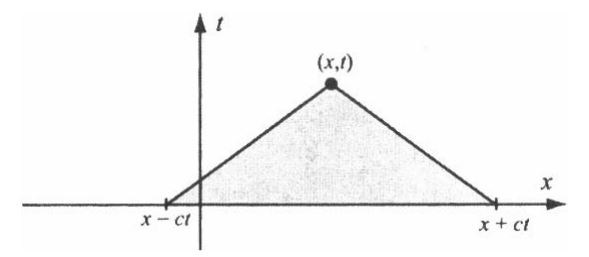
\includegraphics[width=0.6\linewidth]{ch12_6}
	\caption{\textsf{  Illustration of the interval of dependence $[x-ct, x+ct]$ ] (on the x-axis)
for the wave equation on a line. The shaded triangle in the space-time plane (jc/-plane) is
called the domain of dependence. The values of the initial condition functions $\phi(x) and v(x)$ outside of the interval of dependence for $(x,t)$ are irrelevant to the
determination of $u(x,t)$. 
}}
	\label{pfig:ch12_6}
\end{figure}

Although d'Alembert's solution of the wave equation on the infinite string makes
it possible to analyze analytically most of the properties of the solution, the next
variation of a Cauchy problem for the one-dimensional wave equation that we
consider will give rise to analytical formulas that are extremely complicated and
intractable. We now study the wave equation on a string of finite length, which is
fixed at both ends. The precise Cauchy problem that we work with is as follows:
\begin{equation}
V(x)
	\begin{cases} 
(PDE) u_n=c^2 u_{xx}, &  ,0 < x < L, 0< t< \infty ,  u=u(x,t)\\
(BC's)
		\begin{cases}
		u(x,0)=\phi(x), u_t(x,0)=V(x)\\
		u(0,t)=u(L,t)=0
		\end{cases} 
		& ,0 < x < L, 0\leqslant t  < \infty
	\end{cases}
\end{equation}

A model to help visualize this Cauchy problem would be the motion of a guitar
string of length L that is fixed at both ends. What makes a nice analytical formula
impossible here is the fact that once the disturbances reach the ends of the string,
they will bounce back, and things will continue to get more complicated as time
goes on.

Theoretically, we can solve (11) by using d'Alembert's solution for the infinite
string in a clever way. The useful artifice that will be used is called the \textbf{method of
reflections} We first extend the functions $\phi(x) and V(0)$  to be functions on the
whole real line, based on their values in the interval $ 0< x < L$  Labeling these
extensions as $\hat{\phi}(x) and \hat{V}(x)$ ), respectively, they will be created so that they are
odd functions across both of the boundary values $x = 0 and x = L$. Analytically,
this means that

\begin{equation}
\hat{\phi}(-x)= -\hat{\phi}(x) ~~~and~~~ \hat{\phi}(2L - x) = -\hat{\phi}(x),~~~ -\infty < x<\infty
\end{equation}
and the corresponding identities for $\hat{V}$ It can be easily verified (Exercise 14)
that the following formula gives such an extension $-\hat{\phi}(x)$ of $\hat{\phi}(x)$.
\footnote{ Technically, this definition does not define
$\hat{\phi}(x)$ for $x=0, \pm L, \pm L, \cdots .$ The original function $\phi(x)$ ) was also not defined at the endpoints x = 0, and x = L. This was only for notational convenience
in the boundary conditions of (11). The boundary conditions corresponding to the ends of the string
being fixed would force   $\phi(0) = \phi(L)$ = 0 so we extend the definition $\hat{\phi}(x)$ to all real numbers by
specifying $\hat{\phi}$ for $\hat{\phi}(0)=\hat{\phi} (\pm L) =\hat{\phi}(\pm L) = \cdots =0.$  The resulting function will be continuous (otherwise the
string would be broken). }

\begin{equation}
\hat{\phi}(x)
	\begin{cases} 
\phi (x)   ~~~ if~~~ 0< x< L\\
-\phi (-x) ~~~ if ~~~ -L < x <0\\
Extend to be periodic of period 2L\\
\end{cases}		
,0 < x < L, 0\leqslant t  < \infty	
\end{equation}
See Figure 12.7 for a graphical depiction of this construction. An analogous
formula is used to construct $\hat{V}(x)$.\\
\\
EXERCISE FOR THE READER 12.3: (Constructing an M-file for a Periodic
Function) (a) For the function $\phi(x) = 1-|1-x|$ on the interval [0, 2] (L = 2).
Write an M-file, called \texttt{y=phihat(x) } that extends the given ftinction to $-\infty < x<\infty$  by the rule of (13). Try to write your M-file so that it does not use
any loops.
\\
(b) Get MATLAB to plot the graph of your \texttt{phihat(x)} on the interval  $-6\leqslant x \leqslant 6$\\

If we solve the corresponding Cauchy problem (9) on the whole real line using as
data the extended functions $\hat{\phi}(x)$ and $\hat{V}(x)$ d v(x) for boundary data, the ftinction $\hat{u}(x,t)$ that arises will, in fact, extend the solution of (11). 


\begin{figure}[H]
	\centering
	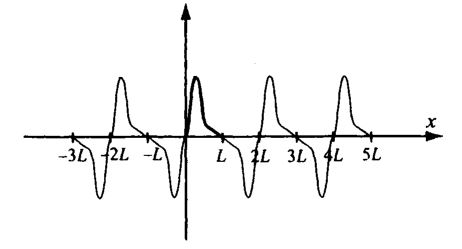
\includegraphics[width=0.6\linewidth]{ch12_7}
	\caption{\textsf{  Illustration of the extension (13) of a function $\phi(x)$ ) defined from x = 0 to x
= L (heavy graph portion) to a ftinction $\hat{\phi}(x)$. that is odd about each of the endpoints x = 0
and x - L }}
	\label{pfig:ch12_7}
\end{figure}
Some parts of this assertion are clear. Defining $u(x,t) = \hat{u} (u,t)$ for $ 0\leqslant \leqslant L$ and $ t\geq 0$  (i.e., take u to be the function ü restricted to the domain of the 
problem (11)), it is clear that u{x,t) satisfies the wave equation and the first two 
(initial) boundary conditions since $\hat{u}$ does. Because of the odd extension 
properties of $\hat{\phi}$ and $ \hat{v} (x)$ 
\\
\\
\textbf{EXAMPLE 12.2:} \textit{(A Plucked Guitar String)} 
Consider what happens to a guitar string of length 4 units that is plucked with one finger as shown in Figure 12.8 and then released (at time  $t = 0$). Assume that the units are chosen so that wave speed $ c=(1/ \rho )^1/2 $ equals 1. By using the method of reflections, get MATLAB to create a series of snapshots of the wave profiles for each of the 12 times starting with time t = 0 and advancing to t = 6 in increments of 0.5. 
\begin{figure}[H]
	\centering
	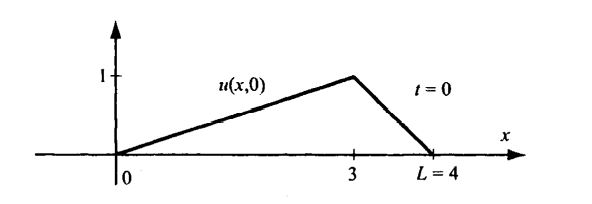
\includegraphics[width=0.6\linewidth]{ch12_8}
	\caption{\textsf{ The initial profile of the plucked guitar string of Example 12.2.}}
	\label{pfig:ch12_8}
\end{figure}
SOLUTION: Looking at Figure 12.8, we can write: 
\begin{equation}
\phi(x) (\equiv u(x,0)) =
\begin{cases}
x/3, ~~~~~for~ 0 \leqslant x \leqslant 3 \\
4 - x, ~for~ 0\leqslant x \leqslant 3 
\end{cases} .
\end{equation}
Also $V(x)(\equiv W,(JC,0)) = 0$ ince the string is released without velocity. We first 
create an M-file for $ \hat{\phi}(x)$ using a similar construction as was done in the solution 
of Exercise for the Reader 12.3. 
\begin{verbatim}
function y = EX12_2phihat(x) 
if (0 <= x)&(x <= 3), y=x/3; 
elseif (x >=3)&(x<=4), y=4-x; 
elseif (x<0)&(x>=-4), y = -EX12_2(-x); 
else q=floor(<x+4)/8); y=EX12_2phihat(x-8*q); 
end 
\end{verbatim}
We can now use MATLAB to create the desired snapshots. To make for a 
convenient single graphic of all 41 plots, we use the subplo t command to 
partition the plot window into smaller pieces. 
\\
\begin{lstlisting}
function y = EX12_2phihat(x) 
>> counter=l; 
>> x=0:.01:4; 
>> z=zeros (size (x) ) ; will be used to add axes to plots 
>> elf Itreshon up the plot window 
	for t=0:.2:8 
	xl=x+t; x2=x-t; 
		for i=l:401 
		u(i)=.5*(EX12_2phihat(xl(i))+EX12_2phihat(x2(i))); 
	end 
	subplot(7,6,counter), plot(x,u), hold on 
	plot (x, z, ' k ) adds a central axis to each 	plot 
	axis((0 4 -1 1]) 
	counter=counter+l; 
	hold off 
end
\end{lstlisting}
\begin{figure}[H]
	\centering
	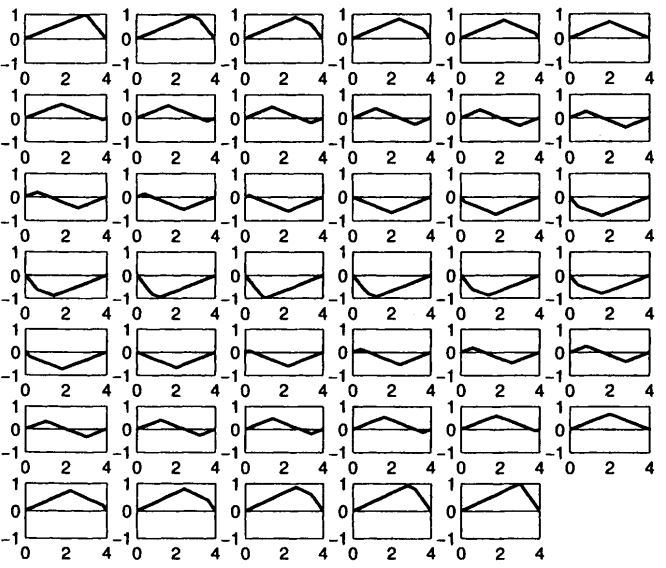
\includegraphics[width=0.8\linewidth]{ch12_9}
	\caption{\textsf{ The initial profile of the plucked guitar string of Example 12.2.}}
	\label{pfig:ch12_9}
\end{figure}
\textbf{FIGURE 12.9}: Snapshots of the plucked guitar string of Example 12.2. (To be read from 
left to right, and then top to bottom.) The speed of the wave is taken to be one unit length 
per unit time. Each successive square represents an increment of 0.2 units of time. Notice 
that the last frame corresponds to eight units of time and is exactly the initial profile. 
\\
\\
Analytically, the waves that result on such finite strings are quite messy to 
describe. Physically, what is happening is that two waves are still moving in 
opposite directions at speeds equal to c. Each is constantly bouncing off the ends, 
reflecting and superimposing with the other. To get a better idea of the properties of the solution, it is a good idea to create a MATLAB movie for it (Exercise 4). 
Further details in this area can be found in Section 3.2 of [Str-92].
\\
\\
EXERCISE FOR THE READER 12.4: Prove that the solution of the wave 
problem on the finite string (11) is always periodic in the time variable with period 
Lie.\\
\\
\textbf{Suggestion:} Use the solution arising from the method of reflections.\\
EXERCISE FOR THE READER 12.5: {Single Pulse Wave on a Finite String) 
Consider the wave problem (11) with c = 2, and initial profile $\phi(x)$ given as in 
Figure 12.10. Obtain a series of snapshots from time / = 0 through t = 10 in 
increments of 0.5 of the solution of the problem (11) under the hypotheses that:  
\\
(a) The impulse is moving to the right initially with speed 2 units per unit of time.
\\ 
(b) The impulse is moving to the right initially with speed 1 unit per unit of time.
\\ 
(c) The impulse is moving to the right initially with speed 4 units per unit of time.
\\
You need not worry about finding an extremely accurate analytical formula to 
model the initial profile  $\phi(x)$(x); you can simply use polynomial interpolation (as in 
Section 7.4) with or without derivative conditions. 
\begin{figure}[H]
	\centering
	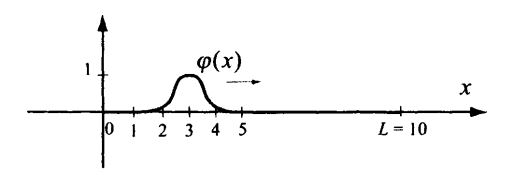
\includegraphics[width=0.8\linewidth]{ch12_10}
	\caption{\textsf{Initial profile for the impulse wave of Exercise for the Reader 12.5. The 
impulse is moving to the right. }}
	\label{pfig:ch12_10}
\end{figure}
Waves (i.e., solutions of the wave equation) satisfy a conservation of energy 
principle that is very important in physics. We demonstrate this principle for the 
one-dimensional wave equation written in physical form: $\rho u_u = Tu_{ss}$, where, we recall, $ \rho $ is the mass density of the string and $T$ is the tension. From physics, the 
\textbf{kinetic energy} of a mass m, which is moving at a velocity $v$, is defined to be $\dfrac{1}{2}mv^2$. Breaking the wave into infinitesimal segments, this gives rise to the 
definition: 
\begin{equation}
KE(t)=\dfrac{1}{2} \rho \int_a^b u_t (x,t)^2 dx ~~~~~~~~~~~~ t\geq 0, 
\end{equation}
for the kinetic energy of the string at time /. This improper integral will converge 
under most reasonable physical assumptions. For example, if both of the initial 
condition functions  $ \rho (x), V(x)$ ) vanish outside a finite interval, so will the 
integrand (but with a larger interval determined by the intervals of dependence). If we differentiate this kinetic energy function with respect to /, we may differentiate 
under the integral sign to obtain: 
Using the PDE to substitute $ Tu_{xx}$for $\rho u_u$ in the above integral, and then 
integrating by parts, we obtain: 
\footnote{ Such differentiations are permissible under general circumstances. Here is a relevant theorem: 
Suppose that $f(x,t)$ is a continuous function of two variables in some rectangular region in the xt-plane:$a\leqslant x\leqslant b, c\leqslant t \leqslant d$ Suppose also that the partial derivative $f,(x,t)$ is continuous in this same 
. b b region. Then the following identity is valid for any t, $c\leqslant t \leqslant d : \dfrac{d}{dt} \int_{a}^{b} f(x,t)dx=\int_{a}^{b} f_t (x,t) dx$. Note that 
although the integral in (14) is over the whole real line, if $\phi(x), V(x)$ vanish outside a finite interval, 
the integral can be evaluated over a finite interval and the theorem can be applied. The theorem can 
even be extended to certain improper integral settings and in cases where the continuity assumptions 
break down at isolated singularities. See any good book on advanced calculus for details on this 
theorem and related results, for example, [Rud-64], [Ros-96], or [Apo-74]. } 
\begin{equation}
\frac{d}{dt} KE(t)=\rho \int_{-\infty}^{\infty} u_t u_u dx ~~~~~~~~~~~~ t\geq 0
\end{equation}
Using the PDE to substitute $Tu_{xx} for \rho u_u$ in the above integral, and then 
integrating by parts, we obtain:
$$
\frac{d}{dt} KE(t)=T \int_{-\infty}^{\infty} u_t u_{xx} dx=Tu_t u_x \int_{-\infty}^{\infty} -T \int_{-\infty}^{\infty} u_{tx} u_x dx =-T \int_{-\infty}^{\infty} u_{tx} u_x dx,
$$
the last equation being valid since the integrated term vanishes off a finite interval. Since $u_{tx} u_x = \partial / \partial t \frac{1}{2} u_x^2$ we may write (again using the differentiation under the 
integral sign rule):
\begin{equation}
\dfrac{d}{dt} KE(t)= -\dfrac{d}{dt}  \dfrac{1}{•2} Tu_{x}^{2} dx, ~~~~~~t\geq 0.
\end{equation}
In basic physics, the \textbf{potential energy} of an object of mass m located at height h is 
defined to be $mgh$, where $g$ is the gravitational constant. The basic conservation of 
energy principle in elementary mechanical physics states that if no external forces 
other than gravity are present, then the total energy $=$ kinetic energy $+$ potential 
energy remains constant. (Think of when an object falls, its velocity increases so 
its kinetic energy increases and its height decreases so its potential energy 
decreases.) The analogue for the potential energy for the string is the following 
integral: 
\begin{equation}
PE(t)=\dfrac{1}{2} T \int_{-\infty}^{\infty} u_x (x,t)^2 dx ~~~~~~t\geq 0
\end{equation}
and, correspondingly, the \textbf{total energy} is defined to be
\begin{equation}
E(t)=KE(t)+PE(t)=\dfrac{1}{2} \int_{-\infty}^{\infty} [\rho u_t^2 + Tu_x^2] dx ~~~~~~t\geq 0
\end{equation}
The identity (16) states that $\dfrac{d}{dt} KE(t)=-\dfrac{d}{dt} KE(t),$ and it follows from (18) that E'(t) = 0 (i.e., the total energy in the wave remains constant). This is the 
conservation of energy. It is extremely important and noteworthy! Regardless of 
how long we let the string propagate, the total energy E of the configuration will 
remain unchanged. 
\\
\\
\textbf{EXAMPLE 12.3:} (a) Compute the total energy of the plucked infinite string of 
Example 12.1, and (b) of the plucked guitar string of Example 12.2. 
\\
\\
SOLUTION: In light of the conservation of energy, we may simply use the initial 
conditions to evaluate E(0) in each case. In both cases, $u_t(x,0)=v(x)=0$ and $u_t(x,0)=\phi '(x)$.
\\
\\
Part (a):  $E= E(0)= \dfrac{T}{2} \int_{-\infty}^{\infty} u_x^2 dx=\dfrac{T}{2} \int_{-\infty}^{\infty}[\phi '(x)]^2 dx =\dfrac{T}{2}2^2 \cdot 2 =4T$. The tension T is  
not specified in the example, so this is as far as we can take this answer
Part (b): Here, since the string is finite, we similarly obtain:
$$E=E(0)= \dfrac{T}{2} \int_{0}^{4} u_x^2 dx= \dfrac{T}{2} \phi '(x)dx=\dfrac{T}{2}[(1/3)^2 \cdot 3+1^2 \cdot 1]=2T/3$$
There are some interesting similarities and differences of waves in one, two, three, 
and higher dimensions. We first point out that future profiles of one-dimensional 
waves will inherit symmetries in the initial conditions. Such results can be 
obtained from d'Alembert's formula (see Exercise 10). The analogue in higher 
dimensions of such symmetry would be \textbf{radially symmetric} waves. In n space 
dimensions such a wave would be a solution of the wave equation (1): 
$$u_n=c^2 \delta u=c^2(u_{x_1 x_1}+\cdots +u_{x_2 x_2}), ~~~~u=u(x_1,x_2, \cdots, x_n, t) \footnote{Most interesting applications of the wave equation occur in one, two or three space dimensions in 
which cases the customary choices x, y, and z are used in place of $x_1, x_2$ and $x_3$ .}$$
which is expressible in the form w(r,t), where $\sqrt{x_1^2 +x_2^2+ \cdots +x_n^2}$
 is the 
distance to the origin. Thus, a radially symmetric w-dimensional wave is not really 
a function of n + 1 variables (as a general such wave might be) but actually just a 
function of two variables. There are analytical techniques for finding formulas for 
radially symmetric waves, but they involve special mathematical functions (such 
as Bessel functions) and the analysis can get a bit complicated. See, for example, 
[Str-92] for a nice treatment on radially symmetric waves. In two dimensions, 
water ripples provide a nice and telling example of radially symmetric waves. In 
three dimensions, sound waves and electromagnetic (e.g., radio) waves provide 
prototypical examples. If a pebble is dropped in water, the water ripples continue 
to propagate and reproduce themselves. In general, disturbances resulting from two-dimensional waves continue to propagate at a given point of space, once they 
have reached this point. In one and three dimensions, once the disturbance of a 
wave passes by a certain point, the wave is finished there and moves on. In three 
dimensions, however, there is an important difference from one-dimensional 
waves. The intensity of the wave decreases as we move away from the source. 
This can be proved from the conservation of energy. (Once a disturbance from a 
three-dimensional radially symmetric wave reaches a distance R from the source, 
it must cover an entire sphere with the same amount of energy that the wave 
packed on much smaller spheres, and the intensity will be decreased at each point 
on these larger spheres. This argument can be made into a rigorous proof.) In 
higher than three dimensions, radially symmetric waves turn out to have the same 
distorted properties of two-dimensional waves. These facts make it clear that we 
are very fortunate to live in a three-dimensional world. Indeed, if the dimension of 
our world were two or higher than three, than anytime someone spoke, we would 
never stop hearing them. In a one-dimensional world, anytime anyone spoke or a 
noise was made, everyone would hear it and with the same intensity regardless of 
how far away from the source they were! For a rigorous proof that radially 
symmetric distortion-free waves are only possible in one and three dimensions, 
and that only in one dimension are radially symmetric waves possible without loss 
of intensity, we refer the reader to the article (with a rather presumptuous title) by 
Morley [Mor-85] and [Mor-86].  
\\
\line(1,0){\textwidth}
\\
\textbf{EXERCISES 12.1}
\\
\\
\begin{enumerate}
 \item
		(Making Snapshots of Vibrating Strings) For each of the following initial data sets, create a 
series of snapshots of the solution of the wave problem (9): 
$$
\begin{cases} 
(PDE) u_u=u_{xx}, ~~~~~~~ -\infty <x< \infty ,0<t< \infty , u=u(x,t)\\ 
(BCs) u(x,0)=\phi (x) , u_t(x,0)=v(x) ~~~~~~~ -\infty <x <\infty ,0 \leqslant t< \infty '
\end{cases}$$
\\
with c (wave speed) = 1
\\
\\
(a) 
$\phi(x)=
\begin{cases} 
sin(x), for~~ 0 \leqslant x\leqslant 2 \pi \\
0, ~~~~~~~otherwise
\end{cases}$, v(x)=0
\\
(b)
$\phi(x)=
\begin{cases} 
sin(2x), for~~ 0\leqslant \leqslant x\leqslant 2 \pi \\
0, ~~~~~~~~~otherwise
\end{cases}$, v(x)=0
\\
(c)
$\phi(x)=0 , ~~ v(x)
\begin{cases} 
1 , ~~~~~~for~~ 6 \pi  \leqslant 2\pi \leqslant 8\pi\\
0, ~~~~~~~otherwise
\end{cases}$.
\\
(d)
$\phi(x)=0
\begin{cases} 
sin(x), for ~~0 \leqslant x\leqslant 2 \pi \\
0, ~~~~~~~otherwise
\end{cases}$.
$\begin{cases} 
1 , ~~~~~~for~~ 6 \pi \leqslant 2 \pi \leqslant 8\pi  \\
0, ~~~~~~~otherwise
\end{cases}$.
\\
Obtain snapshots for the time range $0\leqslant t \leqslant 14$ in increments of $\bigtriangleup t=2$ , and choose the axes 
range so that the plots show all disturbances of the wave in an informative fashion. 
	\item
			(More snapshots of vibrating strings) For each of the following initial data sets, create a series 
of snapshots of the solution of the wave problem (9): 
$$\begin{cases} 
(PDE) u_u=u_{xx}, ~~~~~~~ -\infty <x< \infty ,0<t< \infty , u=u(x,t)\\ 
(BCs) u(x,0)=\phi (x) , u_t(x,0)=v(x) ~~~~~~~ -\infty <x <\infty ,0 \leqslant t< \infty '
\end{cases}$$
\\
with c (wave speed) = 1. 
\\
(a)
$\phi(x)=0
\begin{cases} 
sin(x), ~~ for~~ 0\leqslant x\leqslant \pi \\
0, ~~~~~~~~~otherwise
\end{cases}$,
$v(x)
\begin{cases} 
-cos(x), ~~for ~~ 0\leqslant x \leqslant \pi \\
0, ~~~~~~~~~~~~~otherwise
\end{cases}$,
\\
(b)
$\phi(x)=0
\begin{cases} 
sin(x), ~~ for~~ 0\leqslant x\leqslant \pi \\
0, ~~~~~~~~~otherwise
\end{cases}$,
$v(x)
\begin{cases} 
-2cos(x), ~~for ~~ 0\leqslant x \leqslant \pi \\
0, ~~~~~~~~~~~~~otherwise
\end{cases}$,
\\
(c)
$\phi(x)=0
\begin{cases} 
sin(x), ~~ for~~ 0\leqslant x\leqslant \pi \\
0, ~~~~~~~~~otherwise
\end{cases}$,
$v(x)
\begin{cases} 
-0.5cos(x), ~~for ~~ 0\leqslant x \leqslant \pi \\
0, ~~~~~~~~~~~~~otherwise
\end{cases}$,
\\
(d)
$\phi(x)=0
\begin{cases} 
sin(x), ~~ for~~ 0\leqslant x\leqslant \pi \\
0, ~~~~~~~~~otherwise
\end{cases}$,
$v(x)
\begin{cases} 
-4cos(x), ~~for ~~ 0\leqslant x \leqslant \pi \\
0, ~~~~~~~~~~~~~otherwise
\end{cases}$,
\\
Obtain snapshots for the time range $0 \leqslant t \leqslant 20$ in unit increments. Physically, explain how the 
four sets of initial conditions are related. 
	\item
		{\textit{(Making Movies of Vibrating Strings)}  For each of the vibrating string problems ((a) through (d)) 
of Exercise 1, create a MATLAB movie of the vibrating string on the time range $0 \leqslant t \leqslant 14$. 
View each at various speeds and repetitions. }
	\item 
		{\textit{(More Movies of Vibrating Strings)} For each of the vibrating string problems ((a) through (d)) 
of Exercise 2, create a MATLAB movie of the vibrating string on the time range $0 \leqslant t \leqslant 20$. 
View each at various speeds and repetitions}
	\item
		(a) Create a MATLAB movie for the guitar string wave of Example 12.2 from time t = 0 till 
time / = 24. View it at various speeds and repetitions. 
(b) Create a MATLAB movie for the single impulse wave of Exercise for the Reader 12.5 from 
time / = 0 till time t = 40. View it at various speeds and repetitions. 
	\item
	{Snapshots of Vibrating Finite Strings) For each of the following initial data sets, create a series 
of snapshots of the solution of the wave problem (11):\\
$$\begin{cases} 
	(PDE) u_u=u_{xx}, ~~~~~~~ 0< x< L, 0<t \infty , u=u(x,t) \\ 
	(BCs) 
\begin{cases}
	u(x,0)=\phi(x) , u)t(x,0)=v(x)\\
	u(x,t)=u(L,t)=0
\end{cases}, 
	0<x<L, 0\leqslant t< \infty '
\end{cases}$$}
with c (wave speed) = 1. 
\\
(a)
$\phi(x)=
\begin{cases} 
	sin(x), for~~ 0\leqslant  x\leqslant 2 \pi \\
	0, ~~~~~~~otherwise
\end{cases}$, 
	$v(x)=0 , L=4 \pi$.
\\
(b)
$\phi(x)=
\begin{cases} 
	sin(x), for~~ 0\leqslant  x\leqslant 2 \pi \\
	0, ~~~~~~~otherwise
\end{cases}$, 
	$v(x)=0 , L=3 \pi$.
\\
(c)
$\phi(x)=
\begin{cases} 
	sin(x), for~~ 0\leqslant  x\leqslant  \pi \\
	0, ~~~~~~~otherwise
\end{cases}$, 
	$\begin{cases} 
		-2cos(x), ~~for~~ 0 \leqslant x \leqslant \pi \\	
		0, ~~~~~~~~~~~~~~~otherwise
	\end{cases}
		L=3 \pi$.
\\
(d)
$\phi(x)=
\begin{cases} 
	sin(x), for~~ 0\leqslant  x\leqslant 2 \pi \\
	0, ~~~~~~~otherwise
\end{cases}$, 
	$\begin{cases} 
		1, ~~for~~ 6\pi \leqslant x \leqslant 8\pi \\	
		0, ~~~~~~~~~~~~~~~otherwise
	\end{cases}
		L=10 \pi$.
\\
\\
Obtain snapshots for the time range $ \vartriangle \leqslant t \leqslant40$ in increments of $\vartriangle t=2$.
	\item
		 \textit{(Making movies of Vibrating Finite Strings)} For each of the vibrating string problems ((a) 
through (d)) of Exercise 6, create a MATLAB movie of the vibrating string on the time range 
$0 \leqslant t \leqslant 60$. View each at various speeds and repetitions.
	\item 
		Compute the total energies of each of the vibrating infinite strings in Exercise 1. 
		\item 
		Compute the total energies of each of the vibrating finite strings in Exercise 6.  
		\item 
		\textit{(Symmetry of Waves on an Infinite String}) Consider the solution of the wave problem (9): 
 $$\begin{cases} 
	(PDE) u_u=c^2 u_{uu}, ~~~~~~~ - \infty< x< \infty, 0<t \infty , u=u(x,t) \\ 
	(BCs) u(x,0)=\phi (x), u_t(x,0)=v(x) ~~~~~~~
	-\infty< x< \infty, 0\leqslant t< \infty 
\end{cases}$$
 Use d'AIembert's formula to prove the following symmetry inheritance results.
 \\ 
(a) If both of the initial data are even functions  of $x (i.e., \phi(-x) = \phi(x) and v(-x) - v(x)$ for 
all x) then so will be the wave profile at any future time: $u(-x>t) = u(x,t)$ for all $x$ and $t \geq 0$ . 
\\
(b) If both of the initial data are odd functions of x $(i.e., \phi(-x) = -\phi(x) and V(-x) = -V(x)$ for 
all x), then so will be the wave profile at any future time: $u(-x, t) = -w(x, t)$ for all $x$ and $t \geq 0$ .
\\ 
		\item 
		\textit{(Waves on a Semi-infinite String)} Consider the solution of the following wave problem similar 
to the finite-string problem (11) except that only one end of the string is held fixed. 
$$\begin{cases} 
	(PDE) u_u=u_{xx}, ~~~~~~~ 0< x< \infty, 0<t \infty , u=u(x,t) \\ 
	(BCs)
	\begin{cases} 
	u(x,0)=\phi (x), u_t(x,0)=v(x)\\
	u(x,t)=0
	\end{cases}
	0<x<\infty, 0\leqslant t< \infty 
\end{cases}$$
(a)Making use of d'AIembert's formula and an appropriate "method of reflections" technique 
similar to that used in the text for the finite string, develop a program for solving this problem. 
We point out that such a method will not be a numerical method, per se, since it will simply use 
the computer to perform analytical computations (and the only errors are due to roundoff). 
\\
(b) Obtain snapshots of profiles of the solution to the above problem using the following initial conditions:
$\phi(x)=
\begin{cases}
	sin(x) for~~ 0\leqslant x \leqslant2 \pi\\
	0, ~~~~~~~otherwise
\end{cases},
	v(x)=0, c=1$
(c) Obtain snapshots of profiles of the solution to the above problem using the following initial 
conditions:
$$\phi(x)=
\begin{cases}
	sin(x) for~~ 0\leqslant x \leqslant2 \pi\\
	0, ~~~~~~~otherwise
\end{cases},
	v(x)=0
	 \begin{cases}
	 	1,~~for ~~~6\pi \leqslant x 8\pi
	 	0,~~~~~~~otherwise
	 \end{cases}
	 	L=10\pi$$
(d) Create a MATLAB movie of the propagation of the wave in part (b). 
\\
(e) Create a MATLAB movie of the propagation of the wave in part (c).
\\
	\item
		\textit{(A Maximum Principle for the Wave Equation)} (a) Suppose that the hypotheses of d'AIembert's 
theorem are satisfied for the Cauchy problem (9): 
$$\begin{cases} 
	(PDE) u_u=c^2 u_{uu}, ~~~~~~~ - \infty< x< \infty, 0<t \infty , u=u(x,t) \\ 
	(BCs) u(x,0)=\phi (x), u_t(x,0)=v(x) ~~~~~~~
	-\infty< x< \infty, 0\leqslant t< \infty
\end{cases}$$
\\
and that $\vert \phi(x) \vert$  for all $x$ and that $\vert \int_{a}^{b} v(s)ds \vert \leqslant L$ for all numbers $a$ and $b$. Show that the solution $u(x,t)$ of the Cauchy problem satisfies the inequality: $\vert u)x,t) \vert \leqslant M+L/2c$  for all $x$ and t in the domain. 
\\
(b) Under what general circumstances can you conclude that the maximum amplitude of the wave is attained at time zero
$(i.e., \vert u(x,t)\vert \leqslant max{\vert K(x,0) \vert: \infty < x < \infty} )$?
\end{enumerate}
\textbf{EXERCISES 12.2}
We begin this section by developing finite difference schemes for the numerical 
solution of the one-dimensional wave problem (11):
$$\begin{cases} 
	(PDE) u_u=c^2u_{xx}, ~~~~~~~ 
	0< x< L, 0<t \infty , u=u(x,t) \\ 
	(BCs)
	\begin{cases} 
	u(x,0)=\phi (x), u_t(x,0)=v(x)\\
	u(x,t)=u(L,t)=0
	\end{cases}
	0 \leqslant x \leqslant\infty, 0\leqslant t< \infty 
\end{cases}$$
on a finite string. Our development works in general if we allow c to be a function 
of $t$ and/or $x: c = c(x,t)$. Physically, this corresponds to modeling a vibrating string 
where its characteristics can change depending on time and space. We have 
already shown that in case c is a constant, d'Alembert's Theorem 12.1 coupled 
with the method of reflections can lead to a practical numerical method for solving 
this problem. Since the method simply evaluates the theoretical solution, it is 
relatively error free and so completely adequate for solving (11) with any sets of 
data. This will allow us to compute the errors of the numerical solutions we obtain 
from the finite difference methods. D'Alembert's solution, however, is specific to 
the wave equation, while the finite difference methods that we introduce can be 
easily adapted to work for more general hyperbolic PDE problems. 
\\
\\
At first glance, the similarity of the wave and Laplace's equation would make it 
seem quite plausible that the same general finite difference discretization would 
work nicely, as we witnessed in the case for elliptic boundary value problems. 
The boundary conditions in (11), however, are different in two major ways: (i) 
The region  
$0 \leqslant x < L, 0 \leqslant t < \infty$
> is no longer a bounded rectangle, but rather a half 
strip extending to infinity in the positive /-direction, (ii) There are two boundary 
conditions on the lower side of the strip rather than one. We will indeed discretize 
the PDE in the analogous fashion to what was done to Laplace's equation (replace 
each second derivative with its central difference approximation), but because of 
(i), we will not be able to set up the problem as a finite linear system (there are 
infinitely many nodes). Instead, we will do what is called a marching scheme, 
where the nodal approximations are computed one time level at a time, moving up 
from $t = 0$.At first glance, this may seem like a better situation, since the number 
of variables and the size of the linear systems will be much smaller than if we 
were to do it all at once, as with the elliptic method. For the most part it is true 
that the computations will generally move faster, but one new issue that we will 
need to confront with such marching schemes is the issue of stability. At each 
step, the local truncation errors will still be very small, but they can compound 
quite quickly to make the numerical solutions meaningless. Fortunately, there are 
some stability criteria that give easy ways to arrange the relative step sizes so that 
the schemes will be stable.
\\
\\
All finite difference methods require that the variables be restricted to finite 
intervals,
\footnote{Thus, in terms of the original variables of the PDE, the regions on which finite difference methods 
can be used to solve problems must be rectangular (if there are two variables, or n-dimensional box 
shapes if there are n variables). Coordinate transforms (such as polar coordinates) can allow for other 
sorts of shapes. One of the key advantages of the finite element methods that we will introduce in the 
next chapter is that they allow the solution of PDE problems on more complicated geometrical 
configurations.}
so we will need to restrict time to some specified range, $0 \leqslant t\leqslant T$. As 
in Chapter 11 (see Figure 11.11), we begin by introducing a grid of equally spaced 
x- and /-coordinates for the rectangular region $0\leqslant x\leqslant L, 0\leqslant t \leqslant T$ :

$$0=x_0 < x_1 <x_2< \cdots<x_{N+1} ~~~~\bigtriangleup x_i \equiv x_i-x_{i-1}=h $$
\begin{equation}
	0=t_0 < t_1 <t_2< \cdots<t_{M+1} ~~~~\bigtriangleup x_i \equiv t_i-t_{i-1}=k
\end{equation}
By using the central difference formulas (see Lemma 10.3) in the wave equation, 
we get the following discretization of it: 
\begin{equation}
	\dfrac{u(x_i,t_{j+1})-2u(x_i,t_j)+u(x_i,t_{j-1})}{k^2}=
	c^2 \dfrac{u(x_i,t_{j+1})-2u(x_i,t_j)+u(x_i,t_{j-1})}{h^2}
\end{equation}
We recall that the truncation errors here are 0($k^2$) and 0($h^2$), respectively. Using the notation: 
$$u_{i,j}=u(x_i, t_j),$$
and introducing the parameter
 \begin{equation}
	\mu =ck/h,
\end{equation}
we may express (20) in the following simplified form:
 \begin{equation}
	u_{i,j+1}-2u_{i,j}+u_{i,j-1}-\mu^2[u_{i,j+1}-2u_{i,j}+u_{i,j-1}]=0
\end{equation}
We next solve this equation for the unique term corresponding to the highest time value to obtain: 
 \begin{equation}
	u_{i,j+1}=2(l- \mu^2)u_{i,j}+ \mu^2[u_{i+l,j}+u_{i-l,j}]-u_{u,j-1}
\end{equation}
for $i = 1,2, ...,N,$ and $y = 1, 2, ..., M$. The endpoint boundary conditions tell us that: 
 \begin{equation}
	.u_{0.j}=0=u_{N,j}, ~~~~ for ~all~j
\end{equation}
It follows from (22) and (23) that we may represent the time level j + 1 functional values in terms of the previous two time level functional values by means of the following tridiagonal linear system: 
\begin{figure}[H]
	\centering
	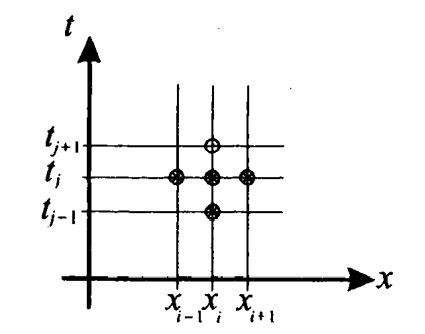
\includegraphics[width=0.4\linewidth]{ch12_11}
	\caption{\textsf{Illustration of the computational stencil for the discretization (20), (21) of 
the wave equation. The single point with largest time coordinate is emphasized, since the 
finite difference method will solve for it using the values of the solution at the previously 
found lower time grid points. }}
	\label{pfig:ch12_11}
\end{figure}








Such a scheme is referred to as an explicit three-level scheme, explicit since the 
highest $(t = (j + 1) l) $ level values are explicitly solved in terms of the lower level 
values; three-level simply means that the nodal values involved in the scheme span 
over three time levels $(t = (J -1)k,jk, (j + 1)k)$. This scheme will progress by 
iterating as we march upward in time. In order to start this recursion, we will 
need the functional values at the first two time levels $t = 0$ and $t = k( = t_1)$. These 
are the two column vectors on the right when j = 1. At time / = 0, these values are specified by the initial condition $u(x,0) = \phi(x)$ (initial wave profile) of (11) and this gives us:
 \begin{equation}
	u_{i,0} =\phi(x_1) ~~for ~~i=1,2,\cdots,N.
\end{equation}
In order to get the required next time level functional values we will need to make 
use of the initial wave velocity condition of (11): $u_t(x,0) = V(x)$. The fact that 
this extra information is actually required (unlike in the elliptic case) is consistent with the fact that the wave problem (11) is well posed. To use this initial velocity to approximate the time level $t = k$ functional values, we will need another difference formula for approximation of derivatives; either the forward or backward difference formulas (Lemma 11.5) will give us what we need. For reasons that will soon be apparent, we choose to use the forward difference 
formula here. 

For a fixed value of JC, and treating u(x>t) as a function of/, the forward difference 
formula implies that:
$$v(x)=u_t(x,0)\thickapprox (u(x,k)-u(x,0))/k\Rightarrow u(x,k) \thickapprox u(x,0)+kv(x)$$
(this is nothing more than the usual tangent line approximation). In terms of our 
grid functional values this translates to: 
\begin{equation}
	u_{i,t} \thickapprox u{i,0}+kv(x_i) ~~for~~i=1,2,\cdots,N.
\end{equation}
Note that (viz. Lemma 11.5) the error of this approximation is $0(k)$, which is of lower order and hence potentially much greater than the $0(h^2+k^2)$ local truncation error for (23). Thus, this lower quality estimate for the / = k time level values (needed to start (23)) could contaminate the overall quality of (23). This problem can be avoided since the approximation can be improved to have error $0(k^2)$ (thus matching those in the foregoing development) if we furthermore assume that the wave equation is valid on the initial line and is sufficiently differentiate. Indeed, based on the differentiability assumption, (the onevariable) Taylor's theorem from Chapter 2 allows us to write: 
$$
u(x,k)=u(x_1,0)+ku_t(x_1,0)+\dfrac{k^2}{6}u_u(x_i,0)+\dfrac{k^3}{6} u_{ttt}(x_i, \hat{k},
$$
where $\hat{k}$ is a number between 0 and k. The assumption that the wave equation is 
valid on the initial line tells us that$ u_u(x,0)=c^2u_{xx}(x,0)=c^2\phi^n(x) $and we are led to the following approximation
\begin{equation}
	u_{i,l}\thickapprox u_{i,0}+kv(x_i)+\dfrac{c^2k^2}{2}\phi^2(x_i) ~~for ~~~i=1,2,\cdots,N,
\end{equation}
with error bound $0(k^2)$.
\footnote{This is the reason we choose to adopt the forward over the backward difference method. We would 
not have been able to make such a local error truncation if we had used the backward difference 
method.}
To avoid computation of derivatives, we may approximate 
$\phi(x_i)$ using the central difference formula: 
$\phi^n(x_i)[\phi (x_{j+l} ) -2\phi(x_i)+\phi(x_{i-1})]/h^2$
(with error $0(h^))$. Installing this approximation into (28) produces the following practical approximating formula for the time level $t = 1$ functional values: 
\begin{equation}
	u_{i,l}=(l-\mu^2)\phi(x_1)+\dfrac{\mu^2}{2}[\phi(x_{i-1})]+kv(x_1)
	 ~~for ~~~i=1,2,\cdots,N,
\end{equation}
which has local truncation error $0(h^2+k^2)$. The next exercise for the reader gives us another way to arrive at the above $0(k^2)$ approximations for $u_{j,l}$ and show it to be valid under slightly different assumptions. 
\\
\\
EXERCISE FOR THE READER 12.6: (a) Use Taylor's theorem to establish the following \textbf{centered difference approximation}: Suppose that $f(x)$ is a function having a continuous third derivative in the interval$ a-h\leqslant x \leqslant a + h$ then the following approximation for $f'(x)$ is valid: 	
\begin{equation}
	f'(x)\dfrac{f(x+h)-f(x-h)}{2h}+O(h^2).
\end{equation}
Note that this is a second-order approximation to $f'(x)$, whereas the forward and backward difference approximation are only first-order approximations. (b) Using the artifice of ghost nodes (introduced in Section 11.4), obtain estimate (29) (with local truncation error $0(h^2 +k^2))$ under the assumption that the solution $u(x,t)$ of the Cauchy problem (11)extends to have a continuous third order time derivative for $t \geq -k$.
\\ 
\textbf{Suggestion:} For part (b), introduce a line of nodes at level $t = -k$ and denote the ghost values of u on these nodes by $u_{i,l}$. The centered difference approximationgives the estimate $u_{i,l}-u_{i,-l}\thickapprox 2kv(x_i) $ that has error $0(k^2)$. 
\\

Even with all of the above attention to detail in developing a finite difference method with $0(h^2+k^2)$ local truncation error, stability issues can seriously corrupt the method. The next example will give good evidence of how badly 
things can go. 
\\
\textbf{EXAMPLE 12.4:} \textit{(Illustration of Instability)} Consider the following Cauchy 
problem of a long plucked string: 
$$\begin{cases} 
	(PDE)u_u=4u_{xx}, ~~~~~~~ - \infty< x< \infty, 0<t \infty , u=u(x,t) \\ 
	(BCs) u(x,0)=\phi (x), u_t(x,0)=v(x) ~~~~~~~
	-\infty< x< \infty, 0\leqslant t< \infty ' 
\end{cases}$$
where $\phi(x)$ is as in Example 12.1 (Figure 12.4). Note this problem is identical to the problem of Example 12.1 except that the wave speed has changed from $c = 1$ to $c = 2$. By D'Alembert's solution (Theorem 12.1), we know the exact solution of this problem is given by (from (10)):
$$u(x,t)=\dfrac{1}{2}[\phi(x+2t)+\phi(x-2t)]$$ 
and the solution will look just like the one shown in Figure 12.5, except now the speed is doubled. Thus, for any specified range of time values, we can view this problem as taking place on a finite string centered at $x = 0$ of sufficiently large length.
\\
(a) Apply the above finite difference scheme (22) with $h = k = 1$ up to time level $t = 5k(= 5)$, and $-12 \leqslant x \leqslant 2$ . To isolate just the effectiveness of (22), use the exact values for the time level $t = k$ values, as determined by D'Alembert's solution, in place of (28). Examine the u-values and compare with those of the exact solution (cf. Figure 12.5). 
\\
(b) Repeat Part (a) with $ = k = 0.1$ up to time level $t = 50k (= 5)$.
\\ 
(c) Repeat Part (a) with $h = 1, k = .5$ up to time level $t = 10k (= 5)$.
\\
\\
SOLUTION: Part (a): With $c = 2$, we have, by (21), $\mu = ck/h = 2$ , so that (23) becomes: 
$$u_{i,j+1}=-6u_{i,j}+4[u_{i+l,j}+u_{i-l,j}]-u_{i,j-1}$$
Since $h = 1$, we get $x_0 = -12, x_{12} = 0, x_{25} = 12$ so by (10) (exact solution), we may write
\\
$u_{i,0}
	\begin{cases}
		2, ~~i=12\\
		0, ~~othervise
	\end{cases}$ and
$u_{i,0}
	\begin{cases}
		1, ~~i=12\pm 2\\
		0, ~~othervise
	\end{cases}$. 
Note that by (22), the of indices with nonzero w-values can advance only one index to the left/right with each new time level. The following MATLAB loop will produce the needed nonzero w-values up to time level $t = 5k$. The instability is so severe that it is  convenient to view the matrix of values. In creating the $6\times 25$ matrix of nodal values, we let the bottom row correspond to the time level zero values and so the top row corresponds to the $t = 5$ values. Note this requires us to modify the of (23) accordingly in our MATLAB code below: 
\begin{lstlisting}
>> U=zeros(6,25); U(6,12)=2 ; U(5,[1 0 14])=1 ; 
>> for j=5:-l: 2 
	   for i=2:2 4 
		    U(j-l,i)=-6*U+4*[U(j,i+l)+U<j,i-l) ]-U(j+l,i);
end 
end 
\end{lstlisting}
The nonzero matrix values are shown below. Note that the actual solution has two 
pulses of height 1 moving from left to right at speed two. The numerical solution 
below is totally off and unstable, it oscillates out of control. Also, the disturbances 
only propagate at speed one. \\
\begin{table}[!ht]
    \centering
    \begin{tabular}{|c|c|c|c|c|c|c|c|c|c|c|c|c|}
    \hline
        256 & -1536 & 4432 & -8048 & 10373 & -10688 & 10424 & -10688 & 10373 & -8048 &4432 & -1536 & 256 \\ \hline
        0 & 64 & -288 & 616 & -812 & 776 & -710 & 776 & -812 & 616 &-288 & 64 & 0\\ \hline
        0 & 0 & 16 & -48 & 67 & -56 & 44 & -56 & 67 & -48 & 16 & 0 & 0\\ \hline
        0 & 0 & 0 & 4 & -6 & 4 & -2 & 4 & -6 & 4 & 0 & 0 & 0 \\ \hline
        0 & 0 & 0 & 0 & 1 & 0 & 0 & 0 & 1 & 0 & 0 & 0 & 0\\ \hline
        0 & 0 & 0 & 0 & 0 & 0 & 2 & 0 & 0 & 0 & 0 & 0 & 0\\ \hline
    \end{tabular}
\end{table}
\\
Part (b): Since c and $ \mu$ are still 2, (22) takes the same form as in part (a), but 
since $x_0 = -12, x_{120} = 0, x_{241} = 12$, and we have
$$u_{i,0}
	\begin{cases}
		2, ~~\vert 120-i\vert /5, ~~ 110 \leqslant i \leqslant 130\\
		0, ~~othervise
	\end{cases}$$
To get uiX, we note that (10) and the initial values give us (since h = k = 0.1) that $u_{i,t}=u_{i+2,0}+u_{i-2,0}$ It is most simple to use a MATLAB loop to compute these values before entering into the main loop based on (23). Using the matrix conventions of part (a), the construction of the matrix of values can be accomplished in MATLAB with the following commands:
\begin{lstlisting}
>>U=zeros(51,251); 
for i=110:130 
	U(51,i)=2-abs(i-120)/5; 
end 
	for i=108:132 
	U(50,i)=U(51,i+2)+U(51,i-2); 
end 
for j=50:-l:2 
	for i=2:250 
		U(j-l,i)=-6*U(j,i)+4MU(j,i + l)+U<j,i-l)]-U(j + l,i); 
	end 
end  
\end{lstlisting}
To see that the numerical solution is still badly unstable, we need only look at the 
middle portion of the last six rows of the matrix (corresponding to the time range: 
$0 \leqslant t \leqslant .5$):


\begin{table}[!ht]
    \centering
    \begin{tabular}{|c|c|c|c|c|c|c|c|c|c|c|}
    \hline
        -45.2 & 416.8 & -842.8 & 1091.2 & -1008.8 & 920 & -1008.8 & 1091.2 & -842.8 & 416.8 & -45.2 \\ \hline
        5 & -19.2 & 71 & -84.8 & 77.8 & -84.8 & 71 & -19.6 & 5 & 616 &-288\\ \hline
        4 & 4.8 & -0/8 & 12.8 & -0.4 & 7.2 & -0.4 & 12.8 & -0.8 & 4.8 & 4  \\ \hline
        3 & 3.6 & 4.2 & 3.2 & 4.6 & 4.4 & 4.6 & 3.2 & 4.2 & 3.6 & 3  \\ \hline
        2 & 2.4 & 2.8 & 3.2 & 3.2 & 3.2 & 3.2 & 3.2 & 2.8 & 2.4 & 2 \\ \hline
        1 & 1.2 & 1.4 & 1.6 & 1.8 & 2 & 1.8 & 1.6 & 1.4 & 1.2 & 1 \\ \hline
    \end{tabular}
\end{table}
Indeed, this shows that even at time level t = 0.5, the profile oscillates rapidly 
between $\pm$1000.
\\
\\
Part (c): Since k is now half of h, we have $\mu = 1$, so that (23) takes the following form:  
$$u_{i,j+1}=u_{i,j+1}+u_{i,j-1}-u_{i,j-1}$$
Since $h = 1$, we get $x_0 = -12, x_{-l2} = 0, x_{25} = 12$ as in part (a), and from (10) (exact solution), we may write
$u_{i,0}
	\begin{cases}
		2, ~~i=12 \\
		0, ~~othervise
	\end{cases}$ and
$u_{i,0}
	\begin{cases}
		1, ~~i=12\pm 1 \\
		0, ~~othervise
	\end{cases}$
Note that  by (23), the set of indices with nonzero w-values can advance only one index to the left/right with each new time level. The construction of the $11 \times 25$ matrix of u-values is done as before and the relevant entries are displayed below. 
\begin{lstlisting}
U=zeros(ll,25);U(11,12)=2; U(10,[11 13])=1; 
for j=10:-l:2 
	for i=2:24 
		U(j-l,i)=U(j,i+l)+U(jf i-l)-U(j+l,i); 
	end 
end 
\end{lstlisting}
\begin{table}[!ht]
    \centering
    \begin{tabular}{|c|c|c|c|c|c|c|c|c|c|c|c|c|c|c|c|c|c|c|c|c|}
    \hline
       1&0&0&0&0&0&0&0&0&0&0&0&0&0&0&0&0&0&0&0&1\\ \hline
       0&1&0&0&0&0&0&0&0&0&0&0&0&0&0&0&0&0&0&1&0\\ \hline
       0&0&1&0&0&0&0&0&0&0&0&0&0&0&0&0&0&0&1&0&0\\ \hline
       0&0&0&1&0&0&0&0&0&0&0&0&0&0&0&0&0&1&0&0&0\\ \hline
       0&0&0&0&1&0&0&0&0&0&0&0&0&0&0&0&1&0&0&0&0\\ \hline
       0&0&0&0&0&1&0&0&0&0&0&0&0&0&0&1&0&0&0&0&0\\ \hline
       0&0&0&0&0&0&1&0&0&0&0&0&0&0&1&0&0&0&0&0&0\\ \hline
       0&0&0&0&0&0&0&1&0&0&0&0&0&1&0&0&0&0&0&0&0\\ \hline
       0&0&0&0&0&0&0&0&1&0&0&0&1&0&0&0&0&0&0&0&0\\ \hline
       0&0&0&0&0&0&0&0&0&1&0&1&0&0&0&0&0&0&0&0&0\\ \hline
       0&0&0&0&0&0&0&0&0&0&2&0&0&0&0&0&0&0&0&0&0\\ \hline
    \end{tabular}
\end{table}
Note the rather surprising results! The result of part (c) quite well represents the actual solution (up to the resolution on the jc-grid). The results of parts (a) and (b) were totally unstable, and despite the fact that the grid of part (b) was much finer (in both variables) than that for part (c), the grid for part (c) turned out to give a much more stable method. It turns out that the relative ratio of $h$ and $k$, not their actual sizes, is what will make or break stability. Such remarkable phenomena did not occur when we applied finite difference methods to elliptic problems in the last chapter. 
\\

The finite difference methods shown above can be proved to converge to the 
exact solution of the wave problem (11) (as the partitions become more and more 
refined) provided that, in addition to the required differentiability assumptions, 
the following Courant-Friedrichs-Levy (CFL) condition holds: 
\begin{equation}
	\mu \equiv ck/h\leqslant1.
\end{equation}
If this condition is violated (i.e., if $\mu > 1$), examples can be constructed where (as in Example 12.4), although all other differentiability assumptions are satisfied, the finite difference approximations will not converge to the exact solution, even as the mesh sizes of both variables tend to zero! In fact when $\mu > 1$, the method is unstable in the sense that errors made at each time stage of the process can significantly affect the subsequent time numerical values. For complete details and proofs on these matters we refer to Section 9.3.1 of [IsKe-66]. The exercises will include an outline of the proof and in the next section we will give some 
details of the analogous theory for the heat equation.
\\

We give here a nontechnical explanation of why such instability can arise. From (23), the numerical values at a new time level at x. depend on those of previous two levels, which lie at most one horizontal step to the left and right of $x_i$. From this we can determine the "numerical interval of dependence" of a grid point $(x_i>t_{j+1})$, analogously to how we defined the interval of dependence of the exact solution (see Figure 12.12). From Figure 12.12, we can see how violation of the  condition can lead to instability of the numerical method. What this amounts to is that the size of the t-steps (= k) is too large relative to the size of the x-steps  h). This means that the numerical interval of dependence (shown by the black double arrowed segment) for ($x_i,y_{j+1}$) is smaller than the theoretical interval of dependence (green arrowed segment). We know from the theory in thelast section that the numerical interval of dependence thus does not take enough information into account to properly formulate the approximations. This can lead to catastrophic results, as we have seen. The diagonally upward black arrows indicate flows of information in the finite difference scheme.
\begin{figure}[H]
    \centering
    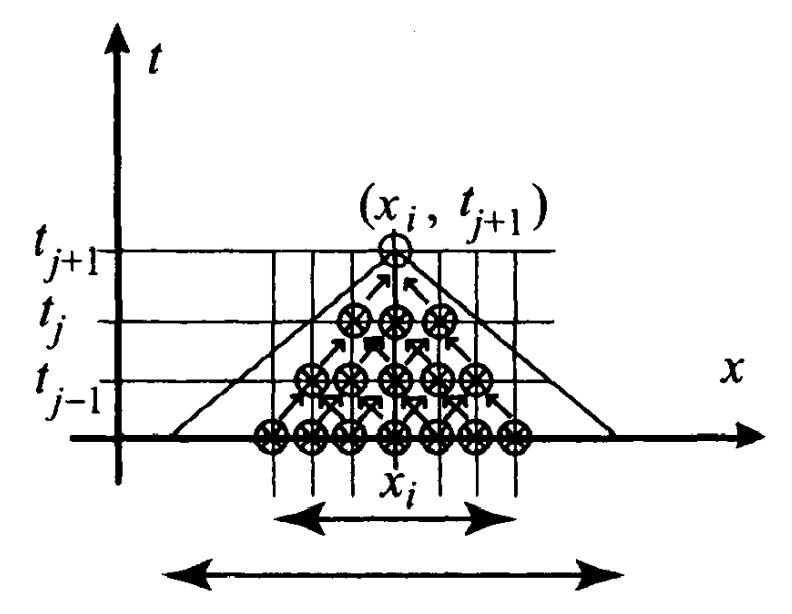
\includegraphics[width=0.6\textwidth]{ch12_12}
   \caption{Illustration of the problem when the Courant-Friedrichs-Levy (CFL) condition is violated}
   \label{fig:ch12_12}
\end{figure}In both parts (a) and (b) of Example 12.4, we had $h = k$, so that (since $c = 2$),  $\mu= $ and the Courant-Friedrichs-Levy conditionis violated. We can see that the numerical wave profiles propagate at only $h$ units (to left and right) for each k unit time level increase. Thus, the numerical profiles cannot keep up with the actual wave propagation (two A units left and right of space for each k unit of time) and the scheme goes haywire. In part (c), however,$ k = h/2$ and now the numerical scheme can keep up, and it does so quite well in that example. It turns out that when the problem is a smooth one, taking step sizes so that $\mu = 1$ can greatly enhance the accuracy of the scheme. It seems quite surprising that for a given (stable) choice of A and $k$, fixing $h$ and decreasing $k$ can sometimes have a detrimental effect on the numerical solution. Shortly, we will introduce an implicit scheme that has better stability properties. 
\\

Recall that the finite difference scheme for elliptic PDEs that we used in the last chapter was implicit and very stable; also, in Part II, we saw that implicit schemes for ODE problems, although more difficult to work with, had better stability properties than explicit schemes. This is a general rule: Implicit schemes are more stable than explicit schemes in numerical differential equations. One advantage of explicit schemes, however, is that many are easily adapted to effectively solve nonlinear problems (provided stability requirements are met). Although we will not enter into any detailed discussion of stability issues for nonlinear PDEs, we will occasionally try to adapt some of our linear schemes to solving nonlinear problems. Often this is what is done in practice. Indeed, a nonlinear problem, when looked at locally (in a small portion of the domain), can be approximated by a linear problem and the latter one dealt with according to linear schemes. For more on nonlinear PDEs, we cite the reference [Log-94]. A more advanced treatment is given in [Smo-83].
\\

Numerical methods for nonlinear PDEs is an extremely active area of mathematical research. We caution the reader that many reasonable-looking finite difference schemes may do poorly for a given nonlinear problem. In general those that are based on conservation laws (physical principles) are the most successful. This seems to imply that a purely mathematical approach to the numerical solution of nonlinear PDEs is not sufficient; an additional requirement is a certain knowledge of the physical principles governing the phenomena that are modeled by the PDEs. For a detailed investigation of such issues, we refer to the two nvolume set [Tho-95a],[Tho-95b]. The book [Dur-99] gives a detailed treatment of various numerical methods for wave (hyperbolic) problems. A particular nonlinear one-dimensional wave equation with a conservation law based finite difference method is nicely examined in [StVa-78].
\\

We now proceed to write a function M-file that will apply the above finite difference scheme to solve a more general version of the wave problem (11) which allows a certain nonlinearity in the PDEs. Specifically, we allow the ends of the wave to have time-dependent variable heights and we allow the coefficient c (wave speed) to depend on /, JC, and/or u. The former conditions mean that we allow forced control on each of the string ends; the more general assumption on c corresponds physically to having a string whose characteristics are not uniform in x (e.g., it could be thicker in some places than in others), are time dependent (e.g., it could weaken or strengthen with time), and even depend on the current position and slope of the string (e.g., the properties of the string may weaken, depending on its composition, in areas where there is a steep slope stretch.) 
\\
\\
In Program 12.1, the main change will be that when we use (29), we need take note of the fact that $\mu -ck/h$ is now no longer (necessarily) constant:  $\mu \mu_{i,j} =c(t_j,x_i,u_{ij},(u_x)_{ij})k/h$. 
In the fourth argument of c we use the centered difference approximation: $(u_x)_{ij}\approx [u_{i,j}-u_{i-1,j}]/2h$. The resulting  (23) will still be an explicit one. 
\\
\\
PROGRAM 12.1: Function M-file for solution of the following wave problem by the finite 
difference method,
\footnote{Although  we have not yet made explicit mention of the incorporation of boundary conditions into 
finite difference schemes for the wave equation, this is a rather obvious extension of ideas presented in 
the previous chapter. Program 12.1 provides an example of such a feature.}

\begin{equation}
	\begin{cases} 
	(PDE) u_n=c(t,x,u,u_x)^2 u_{xx}, ~~0<x<L,~0<t< \infty, ~~u=u(x,t) \\ 
	(BCs)
	\begin{cases} 
	u(x,0)=\phi (x), u_t(x,0)=v(x)\\
	u(x,t)=A(t), ~u(L,t)=B(t)
	\end{cases}
	0<x<L, 0\leqslant t< \infty 
\end{cases}
\end{equation}
This program uses the improved approximation (29) for the level-one time values that work better under greater differentiability hypotheses on the initial data. A more basic program, which uses (27) in place of (29), is left to the following exercise for the reader; it is recommended over this one in case the initial conditions possess singularities. The program assumes that the Courant-Friedrichs-Levy condition has been checked to be satisfied in the region under consideration. 

\begin{lstlisting}
function [x, t, U] = onedimwave(phi, nu, L, A, B, T, N, M, c) 
solves the one-dimensional wave problem u tt - c(t,x,u,u x)N2*u 
Input variables: phi-phi(x) - initial wave profilo function 
nu=nu(x) = initial wave velocity function, L = length of string, 
= Alt) height function of left end of .string u(0,t)=A(t), B=E(t) 
he i gnt function for right end of string u(L, t)-B, T~ final time 
which solution will be computed, N - number of internal x-grid 
values, M - number of internal t-grid values, c -c(t,x,u,u x) -
speed of wave. Functions of the indicated variables must be 
stored as (either inline or M-file) functions with the same 
variables, in the same order. 
Output variables: t - time grid row vector (starts at t-0, ends 
t^T, has M+2 equally spaced values) , x - space grid row vector, 
(M*2) by (M*2) matrix of solution approximations at corresponding 
grid points; y grid will correspond to first (row) indices of U, 
grid values to second (column) indices of U. 
CAUTION: For stability of the method, the Couiant-Friedrichs-Levy 
condition should hold: c(x,t,u,u x)(T/L)(N+l)/(M+l)<1 

h = L/(N+1); k = T/(M+1); 
\end{lstlisting}

\begin{lstlisting}
U=zeros(M+2,N+2); x=0:h:L; t=0:k:T; 
	 Recall matrix indices must start at 1. Thus the 
	 matrix will always be one more than the corrospcn 
	 were used in theoretical development. 
	 
	Assign 1 ef t. and r ight i;i r i.oh 1 et boundar y va 1 ues . 
U(:,l)=feval(A,t)f ; U(:,N+2)=feval (B,t) '; 

	Assign initial time t=0 values and next step t = k v 
for i=2:(N+l) 
	U(l,i)=feval(phi,x(i)); 
	mu(i)=k*feval(c,0,x(i), U(l,i),(feval(phi,x(i+1)) 
l)))/2/h)/h; 
	U(2,i) = (l-mu(i) A2)*feval(phi,x(i) ) +mu (i) A 2/2* (feval(phi,x(i-1))+
...
	feval(phi,x(i+l))) + k*feval(nu,x(i));  	 
end 

	Assign values at interior grid points 
for j=3:(M+2) 
for i=2:(N+l) 
	mu(i)=k*feval(c,t(j),x(i),U(j-l,i), (U (j-1, i + 1) -U ( 
	First form needed tridiagonai matri 
	Tri = diag(2*(l-mu(2:N+l).A 2)) + diag(mu(3:N+1).A 
diag(mu(2:N). A 2 , 1) ; 
	Now perform the matrix multiplications to iterat 
	solution values for increasing time levels. 
	U(j,2: (N+l))*(Tri*(U(j-l,2:(N+l)") ')) '-U(j-2,2: (N+ 
	U(j,2)=U(j,2)+mu(2) A2*feval(A,t(j-1)) ; 
	U(j,N+l)=U(j,N+l)+mu(N+l)A 2*feval(B,t(j-l)); 
end 
end 
\end{lstlisting}
As was implicit in Program 12.1, we point out that the Courant-Friedrichs-Levy (CFL) condition can be expressed using the input parameters in the above M-flle in the following way: 
\begin{equation}
	\mu=c(t,x,u,u_x)\dfrac{T}{•L}(\dfrac{N+1}{M+1})\leqslant 1
\end{equation}
The actual M-file is quite short. In the next example we will test both the accuracy  runtime of this program with a wave problem with nicely smooth input data and whose exact solution is available to compute errors. It will also demonstrate some interesting pathologies when played against the Courant-Friedrichs-Levy condition. 
\\
\\
\textbf{EXAMPLE 12.5:} Use Program 12.1 to solve the following wave problem on the time interval $0 \leqslant t \leqslant 2$: 
$$\begin{cases} 
	(PDE) U_{tt}=u_{xx}, ~~~~~~~~~~~~~~~~~ 0<x\pi , 0<t<\infty, u=u(x,t)\\ 
	(BCs)
	\begin{cases} 
	u(x,0)=sin x, u_t(x,0)=0\\
	u(x,t)0, ~~ u(\pi , 0)=0
	\end{cases}
	0<x<\pi, 0\leqslant t< \infty 
\end{cases}$$
using the following grid sizes. In each case, compare the results with the actual solution $u(x,t) = cos t sin x$ on the indicated time levels. If the graphs are too close to discern differences, compute the maximum error numerically.
\\
(a) $N= 10, M= 15$. Note that this set of parameters slightly violates the Courant-Friedrichs-Levy condition. Compare the numerical solution with the exact solution at time levels $t = 0.5, t = 1, t = 1.5, t = 2$. 
\\
(b) $N = 10, M = 29$. Note that this set of parameters satisfies the Courant-Friedrichs-Levy condition. Compare numerical solution with exact solution at time 
levels $t = 4$ and $t= 8$. 
(c) $N = 100, M - 15$. Note that this set of parameters strongly violates the Courant-Friedrichs-Levy condition (31) $(\mu = 16.0746)$.
\\
\\
SOLUTION: We create three sets of data for each of the three sets of parameters and label them differently for future use. 
\\

We first create inline functions for the initial data of this wave problem:

 
\begin{lstlisting}
>>phi = inline('sin(x)'); 
>>nu= inline ('0'); A=nu; B=A; c=inline('1', 't,'x','u', 'ux'); 
	nu = Inline function: 
		nu(x) = 0
\end{lstlisting}
 
We now create the numerical solutions for each of the three parts: 
\begin{lstlisting}
>> (xl, tl, Ul] = onedimwave(phi, nu, pi, A, B, 8, 10, 15, c) ; 
>> [x2, t2, U2] = onedimwave(phi, nu, pi, A, B, 8, 10, 29, c); 
>> fx3, t3, U3] = onedimwave(phi, nu, pi, A, B, 8, 100, 15, c) ;
\end{lstlisting}
Part (a): To produce the desired snapshots, we take note of the general relationships between $t$ and $j$: $k=\dfrac{2}{M+1}, t_j=jk=\dfrac{2j}{M+1}$ so $j=\dfrac{(m+1)t_j}{2}$.
Thus, when M = 15, we have y = 8ry, so the values f = 0.5, 1.0, 1.5, and 2.0 correspond respectively to the indices $y = 4, y = 8, y = 12$ and $j = 16$. Since the MATLAB indices are one greater than these actual indices, we may create and plot the desired numerical snapshots as follows: 

\begin{lstlisting}
>> subplot(1,4,1) 
>> plot(xl, Ul(5, :)), axis([0 pi -1 l]),hold on 
>> plot(xl, cos(2)*sin(xl),'r') 
>> subplot(l,4,2) 
>> plot(xl, Ul(9, :)), axis([0 pi -1 l]),hold on 
>> plot(xl, cos(4)*sin(xl),'r') 
>> subplot(l,4,3) 
>> plot(xl, Ul(13, :)), axis([0 pi -1 l]),hold on 
>> plot(xl, cos(6)*sin(xl),'r') 
>> subplot(1,4,4) 
>> plot(xl, Ul(17, :)), axis([0 pi -1 l]),hold on 
>> plot(xl, cos(8)*sin(xl),'r') 
\end{lstlisting}
We have set the axes to an appropriate setting for comparisons and used the horizontal stacking of the subplot so as to make the vertical errors more detectable. 
The resulting graphic is shown in Figure 12.13.

\begin{figure}[H]
	\centering
	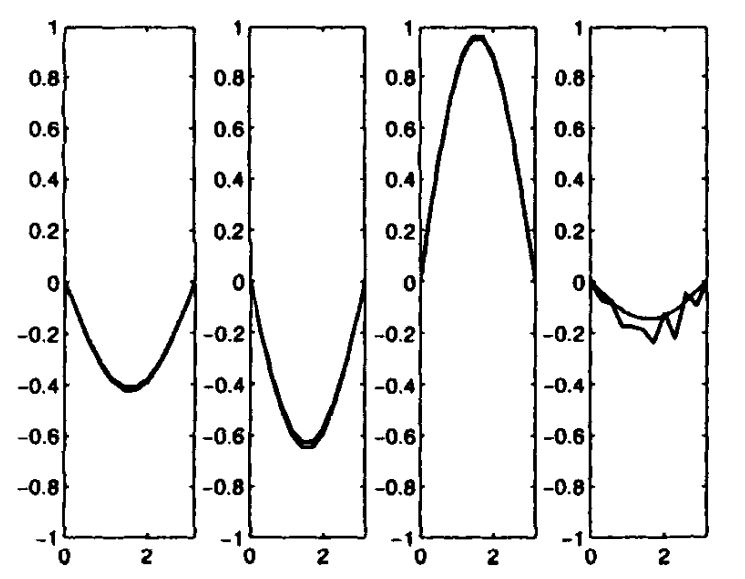
\includegraphics[width=0.6\linewidth]{ch12_13}
	\caption{\textsf{Comparison of the computed finite difference solution's snapshots jagged) with the actual solution's snapshots (smooth) for the wave problem of Example 12.5. The four plots correspond to snapshots at  levels $t = 0.5, t = 1, t = 1.5, t = 2$, respectively. The numerical solution was obtained using $N=10$ interior grid points for x and M- 15 interior grid points for $x$, which resulted in a violation of the Courant-Friedrichs-Levy condition (31) with $\mu = 1.75... > 1$. All except the last profile show the numerical snapshots to be reasonably decent with only small errors that are  visible to the naked eye. At $t = 2$, however, the numerical graph starts to break its pattern and relative errors reach orders of magnitude of $100\%$. Time levels (from left to right) are $t = 0.5, t = 1, t = 1.5$, and $t =2$}}
	\label{pfig:ch12_13}
\end{figure}


Part (b): In this case, if we plot (as in part (a)) and compare the numerical solution with the actual solution, the results are indistinguishable at both time levels / = 1 and t = 2. To compute the maximum absolute values of the differences, using again the index relation $j=\dfrac{(m+1)t_j}{2}$ (and adding one to j to get MATLAB's indices) we enter the following commands: 

\begin{lstlisting}
>> max(max(abs(U2(:,16)'-cos(4)*sin(x2)))) 
->ans = 0.00131359012313 

>>max(max(abs(U2(:,31)'-cos(8)*sin(x2)))) 
->ans = 0.00343796574347 
\end{lstlisting}
The results are rather accurate considering the somewhat large step sizes (especially in t).
\\
Part (c): Plotting the numerical solution's snapshot at time level / = 2 is accomplished with the command:

\begin{lstlisting}
>>plot(x3 , U3(17, :)) 
\end{lstlisting}

The rather surprising result is shown in Figure 12.14.
\begin{figure}[H]
	\centering
	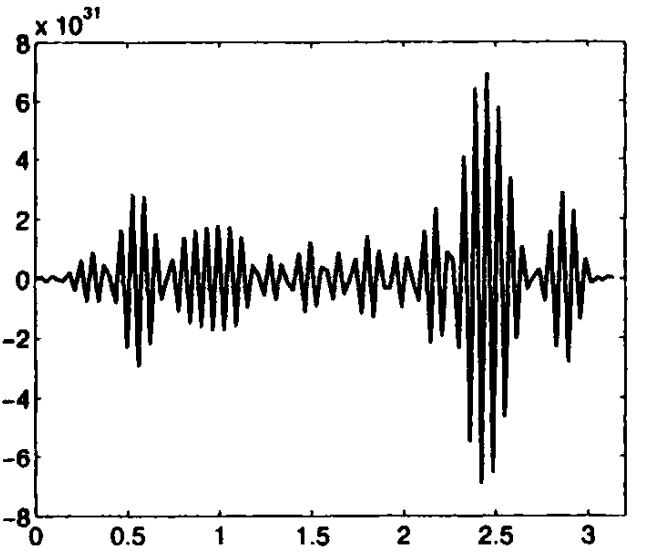
\includegraphics[width=0.5\linewidth]{ch12_14}
	\caption{\textsf{Plot of the snapshot of the numerical solution for part (c) of the wave problem of Example 12.5, using $N= 100$ interior grid points for $x$ and $M= 15$ interior grid points for t, which resulted in a serious violation of the Courant-Friedrichs-Levy condition (31) with $\mu = 16.07... > 1$. Note the amplitude of the graph is 31 orders of magnitude greater than the actual solution, so the result is quite meaningless. Note also that the grid used was actually finer than that used in part (a) (which gave much better results). Thus, blindly refining grids can lead to disastrous results that use more computing time, unless the Courant-Friedrichs-Levy condition is respected.}}
	\label{pfig:ch12_14}
\end{figure}


The next exercise for the reader will show how, with a bit finer of a grid on the time axis (and keeping the same grid on the JC- axis) we can arrive at numerical  with the above program that are numerically indistinguishable from the actual solution. We also point out that the above program is able to handle grids for both x and t with over 1000 points in a reasonable amount of time (a few minutes). This is quite different from the situation for the finite difference methods for elliptic PDEs discussed in the previous chapter. Recall that in the algorithm for elliptic PDEs, it was required to solve a linear system of order roughly $N \cdot M$ to simultaneously solve for the numerical solution at all interior grid values. Numerically solving parabolic equations will also take far fewer computations than do elliptic equations with similar grids, and this is another reason we have grouped hyperbolic and parabolic PDEs together in this chapter. 
\\
\\
EXERCISE FOR THE READER 12.7: 
\\
(a) Modify Program 12.1 into one that uses (27) in place of (29) for the approximation of the function on the level t = k time line. Call this modified function \texttt{onedimwavebasic} . 
\\
(b) Starting with N = 10 interior jt-grid points, begin with Af= 30 interior /-grid points and re-solve the wave problem of Example 12.5, with both the \texttt{onedimwave} program and your newly constructed \texttt{onedimwavebasic} program. Compare with the exact solution at / = 8. Continue to double M (keeping N fixed) until you have completed nine doublings of M Collect the graphs of the resulting errors (at $t = 8$) in a separate $5\times 2$ partitioned (by \texttt{subplot}) window. Repeat with N = 40. Compare and contrast the graphical results, and comment on any observed instability. 
\\

Physically, both hyperbolic and parabolic problems model time-dependent 
. The main difference between them is that while parabolic phenomena are dissipative, solutions to hyperbolic PDEs are conservative. In particular, initial singularities are smoothed out and lost with time under a parabolic PDE and are preserved and propagated under a hyperbolic PDE. Since finite difference schemes tend to average things out (we saw a good example of this in the previous chapter when we showed maximum principles hold for elliptic finite difference schemes), this suggests that finite difference schemes may run into problems for hyperbolic problems with discontinuous data. This is indeed the case, and for this reason, there are other methods that are more suitable for hyperbolic problems with discontinuous data. Examples of alternative methods suitable for hyperbolic problems with singularities include the method of characteristics (the D' Alembert method of the previous section is a special case), and the method of lines. More can be found on such methods in [Abb-66], [Dur-99], and [Ame-77]. Discontinuous data is very natural in hyperbolic problems modeling events such as shocks, explosions, or earthquakes. Our next example will show some typical pathologies that can occur when the finite difference method is applied to a discontinuous problem. 
















\end{document}